\documentclass{article} 
\usepackage{graphicx}
\title{Final Research Document}
\author{Timothy Heidcamp}
\date{March 2016}
\begin{document}
	\maketitle
	
	
	\section{What}
	For my project I will use an N64 controller to give input commands to an Arduino that will change fan a computer fan's speed.   
	
	\section{Why}
	I have chosen these components because I have each item readily available; N64 only has 3 pins--ground, data, and 3.3v; CPU fans work using PWM (Pulse Width Modulation); and the Arduino is easily able to interface with each of these. 
	
	\section{How}
	I will connect the Arduino to the controller using standard test cables and I will power the fan using a battery and control the speed using PWM on the Arduino. 
	
	\section{Challenges}
	Some of the challenges I foresee are...
	\begin{itemize}
		\item issues getting the controller to interface with the Arduino. 
		\item powering the fan with the Arduino
		\item Arduino Assembly is hard...
		\item time constraints...
	\end{itemize}
	
	\section{Solutions}
	The solutions are...
	\begin{itemize}
		\item if I can't interface with an N64 controller I can make my own controller using buttons and variable resisters
		\item I can power the fans using an external source like batteries or a wall adapter. 
		\item I can suck it up and just get the project done.
		\item I realize that I'm working on other projects that are going to require my attention that's why I made this project easy. Should it be too easy I can increase the complexity to a simple game using the remote like Tetris. 
	\end{itemize}
	
	\section{Explanations}
	I don't think I have anything that needs explaining at this point. 
	
	\section{Visualizations}
	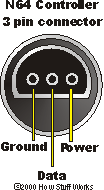
\includegraphics{n64pinout.png}
	
	\section{Sources} 
	http://s.hswstatic.com/gif/n64-pinout.gif
	
	
\end{document}
d